\paragraph{It holds on real objects} On \RealNEvents\ real transients, closed-world information gain was confidently wrong about \RealCCwWhBthree\ of the tidal disruption events, superluminous supernovae and SN~Ibn, so about every second one. Our planner was confidently wrong about \RealCCwWhP\ of them, and it labelled \RealCFlagP\ as unknown (Fig.~\ref{fig:rocreal}). Colour mattered here, since a single band separated the unknowns much less well. On ordinary supernovae, P's accuracy (\RealCAccModP) matched the closed-world planner's (\RealCAccModBthree). We could not prove it was within five points on every noise seed, though, so that hypothesis failed narrowly (Table~\ref{tab:real}).

\begin{table*}[t]
\centering\scriptsize
\caption{Real ZTF replay, preregistered test results per noise seed: estimate [95\% CI]; $^\times$ marks a criterion not met on that seed. CW: confident-wrong rate. $\Delta$: P minus B3, or the colour arm minus the single-band arm for H4. The causal version (v3) is this paper's result. The retrospective version (v2) let planners measure earlier epochs after later ones and is shown only for comparison.}
\label{tab:real}
\begin{tabular}{lll@{\hspace{4pt}}l}
\toprule
& Seed & Causal (v3) & Retrospective (v2) \\
\midrule
H1 $\Delta$CW unmod. & 1 & -0.49 [-0.60, -0.36] & -0.60 [-0.72, -0.49] \\
 & 2 & -0.42 [-0.55, -0.30] & -0.67 [-0.77, -0.56] \\
 & 3 & -0.36 [-0.48, -0.25] & -0.60 [-0.73, -0.48] \\
\addlinespace
H2 AUROC $P(h_0)$ & 1 & +0.81 [+0.76, +0.86] & +0.80 [+0.75, +0.85] \\
 & 2 & +0.81 [+0.76, +0.86] & +0.80 [+0.75, +0.85] \\
 & 3 & +0.79 [+0.73, +0.84] & +0.77 [+0.71, +0.82] \\
\addlinespace
H3 $\Delta$CW mod. & 1 & -0.05 [-0.09, -0.01] & +0.00 [-0.06, +0.07]$^\times$ \\
 & 2 & -0.04 [-0.08, +0.00] & +0.04 [-0.03, +0.10]$^\times$ \\
 & 3 & -0.03 [-0.07, +0.01] & +0.06 [-0.01, +0.12]$^\times$ \\
\addlinespace
H4 $\Delta$AUROC colour & 1 & +0.19 [+0.13, +0.24] & +0.19 [+0.14, +0.24] \\
 & 2 & +0.18 [+0.12, +0.23] & +0.21 [+0.16, +0.27] \\
 & 3 & +0.24 [+0.18, +0.30] & +0.15 [+0.10, +0.20] \\
\addlinespace
H5 $\Delta$acc.\ mod. & 1 & +0.01 [-0.05, +0.07]$^\times$ & -0.08 [-0.14, -0.02]$^\times$ \\
 & 2 & +0.03 [-0.04, +0.09] & -0.06 [-0.13, +0.00]$^\times$ \\
 & 3 & -0.01 [-0.08, +0.05]$^\times$ & -0.08 [-0.14, -0.01]$^\times$ \\
\addlinespace
\bottomrule
\end{tabular}

\end{table*}

\begin{figure}[t]
\centering
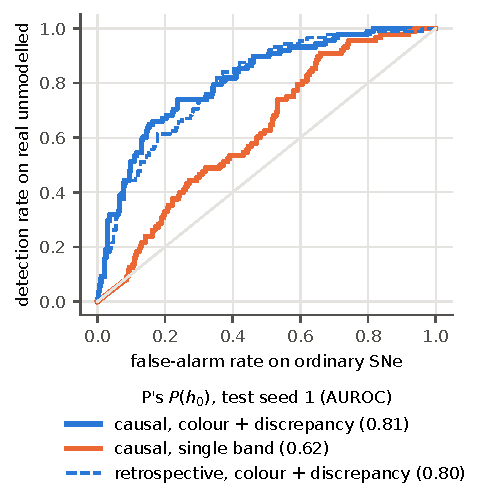
\includegraphics[width=\columnwidth]{generated/figures/fig4_roc_real.pdf}
\caption{Real data. How well $P(h_0)$ separates real unknown transients (TDE, SLSN, SN~Ibn) from ordinary supernovae. Colour plus a model-discrepancy term is what makes it work, and measuring only forward in time leaves the curve almost unchanged.}
\label{fig:rocreal}
\end{figure}

\paragraph{Time order changes the answer} Our first version of this replay let planners go back and measure earlier epochs after later ones, which no spacecraft can do. Once we enforced the time arrow, the planners used far fewer measurements (P \RealCObsP\ of 5, against \RealRObsP\ before), because a one-step utility jumps to a late, informative epoch and gives up the earlier ones. With less data every posterior became less sure, so confident errors fell on both known and unknown events, and P's false ``unknown'' rate on supernovae fell from \RealRFaP\ to \RealCFaP. Two of our conclusions flipped from fail to pass just by respecting causality.
